\documentclass[11pt,letterpaper]{article}
\usepackage[utf8]{inputenc}
\usepackage[spanish]{babel}
\usepackage{graphicx}
\usepackage{hyperref}
\usepackage{listings}
\usepackage{xcolor}
\usepackage{geometry}
\usepackage{titlesec}
\usepackage{enumitem}
\usepackage{float}
\usepackage{caption}
\usepackage{subcaption}

\geometry{letterpaper, margin=2cm}

\titleformat{\section}
  {\normalfont\Large\bfseries}{\thesection}{1em}{}
\titleformat{\subsection}
  {\normalfont\large\bfseries}{\thesubsection}{1em}{}

\definecolor{codegreen}{rgb}{0,0.6,0}
\definecolor{codegray}{rgb}{0.5,0.5,0.5}
\definecolor{codepurple}{rgb}{0.58,0,0.82}
\definecolor{backcolour}{rgb}{0.95,0.95,0.92}

\lstdefinestyle{mystyle}{
    backgroundcolor=\color{backcolour},   
    commentstyle=\color{codegreen},
    keywordstyle=\color{blue},
    numberstyle=\tiny\color{codegray},
    stringstyle=\color{codepurple},
    basicstyle=\ttfamily\footnotesize,
    breakatwhitespace=false,         
    breaklines=true,                 
    captionpos=b,                    
    keepspaces=true,                 
    numbers=left,                    
    numbersep=5pt,                  
    showspaces=false,                
    showstringspaces=false,
    showtabs=false,                  
    tabsize=2
}

\lstset{style=mystyle}

\title{\textbf{Implementación de un Sistema Multijugador para Last Three Standing}}
\author{Proyecto Anna \\ Universidad}
\date{\today}

\begin{document}

\maketitle

\tableofcontents
\newpage

\section{Introducción}

Last Three Standing es un juego de tipo arcade desarrollado en Python utilizando la biblioteca Pygame, donde el jugador controla una nave espacial y debe esquivar y destruir meteoritos. Este proyecto busca ampliar sus características para permitir la modalidad multijugador.

El objetivo principal es transformar la experiencia de juego individual en una experiencia multijugador cooperativa, donde múltiples jugadores puedan unirse a una misma partida. Para lograrlo, se implementará una arquitectura cliente-servidor, donde un servidor desarrollado en Go gestionará la lógica del juego y la comunicación entre los clientes mediante gRPC.

La elección de estas tecnologías responde a necesidades específicas del proyecto:

\begin{itemize}
    \item \textbf{Python con Pygame}: Mantiene la base del cliente por su facilidad para el desarrollo de interfaces gráficas.
    \item \textbf{Go para el servidor}: Aprovecha su rendimiento y soporte nativo para concurrencia.
    \item \textbf{gRPC}: Proporciona un marco de comunicación eficiente y tipado entre lenguajes diferentes.
\end{itemize}

Este informe detalla el proceso de análisis, diseño e implementación del sistema multijugador para Last Three Standing.

\section{Análisis del Problema}

\subsection{Estado Actual del Juego}

El juego Last Three Standing en su versión original es una aplicación monolítica para un solo jugador que ejecuta toda la lógica del juego en un mismo proceso. Sus componentes principales incluyen:

\begin{itemize}
    \item \textbf{Motor del juego}: Gestiona el bucle principal, la detección de colisiones y el renderizado.
    \item \textbf{Gestor de objetos}: Administra la creación, actualización y destrucción de entidades.
    \item \textbf{Gestor de meteoritos}: Controla la generación y comportamiento de los meteoritos.
\end{itemize}

La estructura del código sigue un patrón orientado a objetos con un sistema de eventos para la comunicación entre componentes, pero está diseñada para ejecutarse en un único proceso.

\subsection{Desafíos de la Implementación Multijugador}

La transformación del juego en un sistema multijugador implica afrontar varios desafíos técnicos:

\begin{itemize}
    \item \textbf{Sincronización de estado}: Mantener coherente el estado del juego entre todos los clientes conectados.
    
    \item \textbf{Latencia de red}: Implementar técnicas como la predicción local y la reconciliación para minimizar su impacto.
    
    \item \textbf{Autoridad del servidor}: El servidor debe ser la autoridad final sobre el estado del juego.
    
    \item \textbf{Escalabilidad}: El sistema debe manejar múltiples jugadores simultáneos sin degradar el rendimiento.
    
    \item \textbf{Interoperabilidad}: Garantizar la comunicación eficiente entre el cliente Python y el servidor Go.
\end{itemize}

\subsection{Requisitos del Sistema Multijugador}

Para implementar un sistema multijugador funcional, se han establecido los siguientes requisitos:

\begin{itemize}
    \item \textbf{Conexión y desconexión fluida}: Permitir que los jugadores se unan o abandonen la partida sin afectar a los demás.
    
    \item \textbf{Sincronización de entidades}: Todos los clientes deben ver los mismos elementos en posiciones coherentes.
    
    \item \textbf{Transmisión de acciones}: Las acciones de cada jugador deben reflejarse en todos los clientes.
    
    \item \textbf{Gestión de colisiones}: Las colisiones deben detectarse y procesarse de manera consistente.
    
    \item \textbf{Tolerancia a la latencia}: El juego debe mantenerse jugable incluso con cierto nivel de latencia.
\end{itemize}

\section{Diseño de la Solución}

\subsection{Arquitectura Cliente-Servidor}

Para abordar los desafíos identificados, se ha optado por una arquitectura cliente-servidor con una clara separación de responsabilidades:

\begin{itemize}
    \item \textbf{Cliente (Python)}:
    \begin{itemize}
        \item Renderización de la interfaz gráfica
        \item Captura de entrada del usuario
        \item Predicción local para movimiento fluido
        \item Comunicación con el servidor mediante gRPC
    \end{itemize}
    
    \item \textbf{Servidor (Go)}:
    \begin{itemize}
        \item Gestión del estado autoritativo del juego
        \item Generación y control de meteoritos
        \item Validación de acciones de los jugadores
        \item Detección de colisiones
        \item Difusión de eventos a todos los clientes
    \end{itemize}
\end{itemize}

\begin{figure}[H]
    \centering
    \begin{lstlisting}[language=text]
    +---------------+                 +---------------+
    |               |                 |               |
    |  Cliente 1    |<--------------->|               |
    |  (Python)     |                 |               |
    |               |                 |               |
    +---------------+                 |               |
                                     |               |
    +---------------+                 |   Servidor   |
    |               |                 |     (Go)     |
    |  Cliente 2    |<--------------->|               |
    |  (Python)     |                 |               |
    |               |                 |               |
    +---------------+                 |               |
                                     |               |
    +---------------+                 |               |
    |               |                 |               |
    |  Cliente N    |<--------------->|               |
    |  (Python)     |                 |               |
    |               |                 |               |
    +---------------+                 +---------------+
    \end{lstlisting}
    \caption{Diagrama de la arquitectura cliente-servidor}
\end{figure}

\subsection{Arquitectura del Backend (Servidor Go)}

El backend está implementado en Go, aprovechando sus capacidades de concurrencia para gestionar múltiples conexiones simultáneas.

\subsubsection{Estructura del Servidor}

\begin{figure}[H]
    \centering
    \begin{lstlisting}[language=text]
    +-------------------------------------------------------+
    |                   GameServiceImpl                     |
    |          (Implementación de la API gRPC)              |
    +-------------------------------------------------------+
                           |
                           v
    +-------------------------------------------------------+
    |                     GameServer                        |
    |          (Gestión global del juego)                   |
    +-------------------------------------------------------+
                           |
                           v
    +-------------------------------------------------------+
    |                       Game                            |
    |          (Lógica principal del juego)                 |
    +-------------------------------------------------------+
                  /                   \
                 /                     \
                v                       v
    +-------------------+     +-------------------+
    |   MeteorManager   |     |   ObjectsManager  |
    | (Generación de    |     | (Gestión de       |
    |  meteoritos)      |     |  entidades)       |
    +-------------------+     +-------------------+
    \end{lstlisting}
    \caption{Estructura de componentes del servidor}
\end{figure}

\subsubsection{Componentes Principales}

\begin{itemize}
    \item \textbf{GameServiceImpl}: Implementa la interfaz gRPC definida en el archivo proto.
    
    \item \textbf{GameServer}: Actúa como contenedor principal para el estado global del juego.
    
    \item \textbf{Game}: Implementa la lógica principal del juego.
    
    \item \textbf{MeteorManager}: Gestiona la creación y comportamiento de meteoritos.
    
    \item \textbf{ObjectsManager}: Sistema genérico para gestionar entidades del juego.
\end{itemize}

\subsubsection{Gestión de Concurrencia}

Go ofrece un modelo de concurrencia basado en goroutines y canales que el servidor aprovecha para:

\begin{itemize}
    \item \textbf{Manejo de conexiones concurrentes}: Cada cliente conectado es atendido por una goroutine dedicada.
    
    \item \textbf{Sincronización de estado}: Se utilizan mutexes para proteger el acceso concurrente a datos compartidos.
    
    \item \textbf{Comunicación entre componentes}: Los canales de Go se utilizan para la comunicación asíncrona.
\end{itemize}

\begin{lstlisting}[language=go, caption=Gestión de streams de clientes]
// Estructura para mantener los streams de clientes
type ClientStreamManager struct {
    streams map[string]pb.GameService_SubscribeToEventsServer
    mutex   sync.RWMutex
}

// Difundir evento a todos los clientes
func (m *ClientStreamManager) BroadcastEvent(event *pb.GameEvent) {
    notification := &pb.EventNotification{
        Event:     event,
        Timestamp: time.Now().UnixNano() / int64(time.Millisecond),
    }
    
    m.mutex.RLock()
    defer m.mutex.RUnlock()
    
    for playerID, stream := range m.streams {
        go func(pid string, s pb.GameService_SubscribeToEventsServer) {
            err := s.Send(notification)
            if err != nil {
                log.Printf("Error al enviar evento a %s: %v", pid, err)
            }
        }(playerID, stream)
    }
}
\end{lstlisting}

\subsection{Arquitectura del Frontend (Cliente Python)}

El frontend está implementado en Python utilizando Pygame, adaptado para la comunicación con el servidor.

\subsubsection{Estructura del Cliente}

\begin{figure}[H]
    \centering
    \begin{lstlisting}[language=text]
    +-------------------------------------------------------+
    |                    LastThreeStandingGame              |
    |          (Clase principal y motor del juego)          |
    +-------------------------------------------------------+
                  /               |              \
                 /                |               \
                v                 v                v
    +-------------------+ +------------------+ +------------------+
    |   NetworkClient   | |   MeteorManager  | |  ObjectsManager  |
    | (Comunicación)    | | (Meteoritos)     | | (Entidades)      |
    +-------------------+ +------------------+ +------------------+
            |
            v
    +-------------------------------------------------------+
    |               NetworkEventsManager                    |
    |    (Traduce eventos de red a eventos del juego)       |
    +-------------------------------------------------------+
    \end{lstlisting}
    \caption{Estructura de componentes del cliente}
\end{figure}

\subsubsection{Componentes Principales}

\begin{itemize}
    \item \textbf{LastThreeStandingGame}: Clase principal que extiende el motor base del juego.
    
    \item \textbf{NetworkClient}: Maneja la comunicación con el servidor mediante gRPC.
    
    \item \textbf{NetworkEventsManager}: Actúa como puente entre el sistema de red y el sistema de eventos del juego.
    
    \item \textbf{MeteorManager}: Gestiona los meteoritos en el cliente.
    
    \item \textbf{Player}: Representa al jugador local.
    
    \item \textbf{OtherPlayer}: Representa a los jugadores remotos.
\end{itemize}

\subsubsection{Sistema de Eventos}

El cliente implementa un sistema de eventos para la comunicación desacoplada entre componentes:

\begin{lstlisting}[language=python, caption=Implementación del sistema de eventos]
class GameEngine:
    """Motor base del juego con sistema de eventos."""
    
    def __init__(self, width, height, title, fps=60):
        # ... inicialización ...
        self.event_handlers = {}
    
    def emit_event(self, event_type, data=None):
        """Emite un evento a todos los manejadores registrados."""
        if event_type in self.event_handlers:
            for handler in self.event_handlers[event_type]:
                try:
                    handler(data)
                except Exception as e:
                    print(f"Error en manejador de evento {event_type}: {e}")
    
    def on(self, event_type, handler):
        """Registra un manejador para un tipo de evento."""
        if event_type not in self.event_handlers:
            self.event_handlers[event_type] = []
        self.event_handlers[event_type].append(handler)
\end{lstlisting}

\subsubsection{Predicción y Reconciliación}

Para proporcionar una experiencia fluida a pesar de la latencia de red, el cliente implementa:

\begin{itemize}
    \item \textbf{Predicción de movimiento}: El jugador local se mueve inmediatamente sin esperar confirmación.
    
    \item \textbf{Interpolación}: Para los jugadores remotos, se implementa interpolación suave entre posiciones.
    
    \item \textbf{Extrapolación}: En caso de alta latencia, se predice la posición futura de los jugadores remotos.
    
    \item \textbf{Reconciliación}: Cuando se recibe una actualización contradictoria, se aplica una corrección suave.
\end{itemize}

\section{Interfaces de Comunicación: Protocol Buffers}

La comunicación entre cliente y servidor se realiza mediante gRPC con Protocol Buffers, que proporciona una definición clara y eficiente de las interfaces.

\subsection{Estructura del Archivo Proto}

El archivo \texttt{game.proto} está estructurado en tres partes principales:

\begin{enumerate}
    \item \textbf{Definición de tipos básicos}: Estructuras de datos fundamentales.
    \item \textbf{Definición de mensajes de eventos}: Estructuras para cada tipo de evento.
    \item \textbf{Definición de servicios}: Interfaces RPC que expone el servidor.
\end{enumerate}

\begin{lstlisting}[language=proto, caption=Estructura del archivo game.proto]
syntax = "proto3";

package last_tree_standing;
option go_package = "github.com/user/last_tree_standing/proto";

// Tipos básicos
message Vector2 {
  float x = 1;
  float y = 2;
}

// Mensajes de solicitud y respuesta
message ConnectRequest {
  string player_name = 1;
}

message ConnectResponse {
  bool success = 1;
  string player_id = 2;
  string error_message = 3;
}

// Eventos del juego
message GameEvent {
  string event_type = 1;
  oneof event_data {
    PlayerConnectEvent player_connect = 2;
    PlayerDisconnectEvent player_disconnect = 3;
    PlayerPositionEvent player_position = 4;
    MeteorCreatedEvent meteor_created = 5;
    MeteorDestroyedEvent meteor_destroyed = 6;
    PlayerShotEvent player_shot = 7;
    ScoreUpdateEvent score_update = 8;
  }
}

// Servicios
service GameService {
  rpc Connect(ConnectRequest) returns (ConnectResponse);
  rpc Disconnect(DisconnectRequest) returns (DisconnectResponse);
  rpc UpdatePosition(PositionUpdate) returns (UpdateResponse);
  rpc FireShot(ShotRequest) returns (UpdateResponse);
  rpc SubscribeToEvents(EventsRequest) returns (stream EventNotification);
}
\end{lstlisting}

\subsection{Eventos del Juego}

Los eventos del juego se modelan como un mensaje genérico \texttt{GameEvent} con un campo discriminador \texttt{event\_type} y un campo de datos específico del evento utilizando \texttt{oneof}:

\begin{lstlisting}[language=proto, caption=Definición de eventos del juego]
message GameEvent {
  string event_type = 1;
  oneof event_data {
    PlayerConnectEvent player_connect = 2;
    PlayerDisconnectEvent player_disconnect = 3;
    PlayerPositionEvent player_position = 4;
    MeteorCreatedEvent meteor_created = 5;
    MeteorDestroyedEvent meteor_destroyed = 6;
    PlayerShotEvent player_shot = 7;
    ScoreUpdateEvent score_update = 8;
  }
}

message PlayerConnectEvent {
  PlayerInfo player = 1;
}

message PlayerDisconnectEvent {
  string player_id = 1;
}

message PlayerPositionEvent {
  string player_id = 1;
  Vector2 position = 2;
  float rotation = 3;
}

message MeteorCreatedEvent {
  string meteor_id = 1;
  int32 meteor_type = 2;
  Vector2 position = 3;
  Vector2 velocity = 4;
  float angle = 5;
  float rotation_speed = 6;
}
\end{lstlisting}

\subsection{Servicios RPC}

El servicio principal \texttt{GameService} define las operaciones que los clientes pueden invocar en el servidor:

\begin{lstlisting}[language=proto, caption=Definición del servicio GameService]
service GameService {
  // Conexión y autenticación
  rpc Connect(ConnectRequest) returns (ConnectResponse);
  rpc Disconnect(DisconnectRequest) returns (DisconnectResponse);
  
  // Actualizaciones de estado
  rpc UpdatePosition(PositionUpdate) returns (UpdateResponse);
  rpc FireShot(ShotRequest) returns (UpdateResponse);
  
  // Suscripción a eventos
  rpc SubscribeToEvents(EventsRequest) returns (stream EventNotification);
  
  // Obtención de estado inicial
  rpc GetGameState(GameStateRequest) returns (GameStateResponse);
}
\end{lstlisting}

\subsection{Ventajas de Protocol Buffers y gRPC}

La elección de Protocol Buffers y gRPC para la comunicación cliente-servidor ofrece varias ventajas:

\begin{itemize}
    \item \textbf{Definición clara de interfaces}: El archivo proto actúa como un contrato entre cliente y servidor.
    \item \textbf{Serialización eficiente}: Los mensajes se codifican en un formato binario compacto.
    \item \textbf{Generación automática de código}: Reduce errores y garantiza compatibilidad.
    \item \textbf{Soporte para streaming}: Permite comunicación en tiempo real mediante streams bidireccionales.
    \item \textbf{Interoperabilidad}: Facilita la comunicación entre diferentes lenguajes (Python y Go).
\end{itemize}

\subsection{Flujo de Comunicación}

El flujo típico de comunicación entre cliente y servidor es:

\begin{enumerate}
    \item El cliente se conecta al servidor mediante \texttt{Connect()}.
    \item El cliente establece un stream de eventos mediante \texttt{SubscribeToEvents()}.
    \item El cliente solicita el estado actual del juego mediante \texttt{GetGameState()}.
    \item Durante el juego, el cliente envía actualizaciones de posición mediante \texttt{UpdatePosition()}.
    \item El cliente envía acciones de disparo mediante \texttt{FireShot()}.
    \item El servidor envía eventos a través del stream establecido.
    \item Al salir, el cliente notifica al servidor mediante \texttt{Disconnect()}.
\end{enumerate}

\section{Implementación}

\subsection{Generación de Meteoritos}

Uno de los componentes clave del servidor es el sistema de generación de meteoritos:

\begin{lstlisting}[language=go, caption=Sistema de generación de meteoritos]
// MeteorManager gestiona la creación y comportamiento de meteoritos
type MeteorManager struct {
    game            *Game
    meteors         map[string]*entities.Meteor
    mutex           sync.RWMutex
    nextMeteorID    int
    spawnRate       time.Duration
    lastSpawnTime   time.Time
    difficultyLevel int
}

// Generar un nuevo meteorito con propiedades aleatorias
func (mm *MeteorManager) SpawnMeteor() {
    mm.mutex.Lock()
    defer mm.mutex.Unlock()
    
    // Crear ID único
    meteorID := fmt.Sprintf("meteor_%d", mm.nextMeteorID)
    mm.nextMeteorID++
    
    // Determinar tipo de meteorito según dificultad
    meteorType := mm.selectMeteorType()
    
    // Calcular posición inicial (fuera de la pantalla)
    position := mm.calculateSpawnPosition()
    
    // Calcular velocidad (hacia el centro de la pantalla)
    velocity := mm.calculateVelocity(position)
    
    // Crear nuevo meteorito
    meteor := entities.NewMeteor(
        meteorID,
        meteorType,
        position,
        velocity,
        mm.randomRotation(),
        mm.randomRotationSpeed(),
    )
    
    // Añadir a la colección
    mm.meteors[meteorID] = meteor
    
    // Notificar a los clientes
    mm.game.BroadcastMeteorCreated(meteor)
}
\end{lstlisting}

\subsection{Interpolación en el Cliente}

Para proporcionar una experiencia fluida, el cliente implementa interpolación para los jugadores remotos:

\begin{lstlisting}[language=python, caption=Implementación de interpolación para jugadores remotos]
class OtherPlayer:
    """Representa un jugador remoto en el cliente."""
    
    def update(self, delta_time):
        # Interpolación suave hacia la posición objetivo
        if self.target_position:
            # Calcular factor de interpolación
            self.lerp_factor += self.lerp_speed * delta_time
            if self.lerp_factor > 1.0:
                self.lerp_factor = 1.0
            
            # Interpolar posición
            dx = self.target_position[0] - self.x
            dy = self.target_position[1] - self.y
            self.x += dx * self.lerp_factor
            self.y += dy * self.lerp_factor
            
            # Actualizar velocidad para extrapolación
            self.speed_x = dx * self.lerp_speed
            self.speed_y = dy * self.lerp_speed
        else:
            # Extrapolación basada en velocidad cuando no hay actualizaciones
            self.x += self.speed_x * delta_time
            self.y += self.speed_y * delta_time
\end{lstlisting}

\section{Pruebas – Ejecución}

\begin{figure}
    \centering
    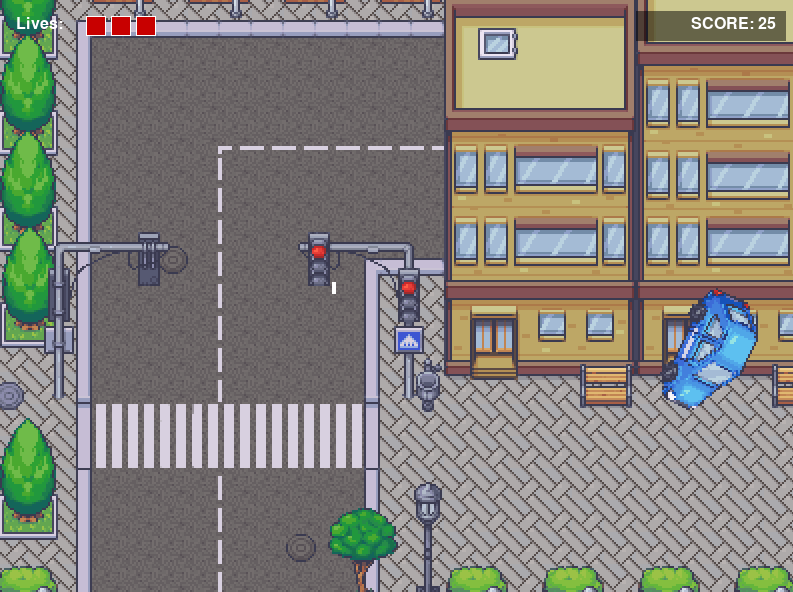
\includegraphics[width=0.5\linewidth]{images/image_game_1.png}
    \caption{Captura del juego}
    \label{fig:enter-label}
\end{figure}

Las pruebas del sistema multijugador se dividieron en varias etapas:

\subsection{Pruebas Unitarias}

Se realizaron pruebas unitarias para verificar componentes individuales:

\begin{itemize}
    \item \textbf{Serialización/deserialización}: Conversión de datos entre Python y Go.
    \item \textbf{Gestión de eventos}: Propagación correcta de notificaciones.
    \item \textbf{Lógica de juego}: Física de movimiento, colisiones y generación de meteoritos.
\end{itemize}

\subsection{Pruebas de Integración}

Las pruebas de integración se enfocaron en la comunicación entre cliente y servidor:

\begin{itemize}
    \item \textbf{Conexión y desconexión}: Proceso de unirse y abandonar una partida.
    \item \textbf{Sincronización de estado}: Coherencia del estado entre clientes.
    \item \textbf{Propagación de eventos}: Reflejo correcto de eventos en todos los clientes.
\end{itemize}

\subsection{Pruebas de Latencia}

Para simular condiciones de red reales, se realizaron pruebas con diferentes niveles de latencia:

\begin{itemize}
    \item \textbf{Latencia baja (50-100ms)}: Experiencia fluida sin ajustes significativos.
    \item \textbf{Latencia media (100-200ms)}: La predicción local compensó adecuadamente los retrasos.
    \item \textbf{Latencia alta (200-500ms)}: Algunas correcciones visibles, pero el juego seguía siendo jugable.
\end{itemize}

\section{Conclusiones}

La implementación de un sistema multijugador para Last Three Standing representa un avance significativo en la evolución del juego, transformándolo de una experiencia individual a una colaborativa. Este proyecto ha demostrado los siguientes puntos clave:

\begin{itemize}
    \item \textbf{Arquitectura efectiva}: La arquitectura cliente-servidor ha demostrado ser efectiva para sincronizar el estado del juego entre múltiples jugadores.
    
    \item \textbf{Comunicación eficiente}: gRPC y Protocol Buffers han proporcionado un mecanismo de comunicación eficiente y tipado entre Python y Go.
    
    \item \textbf{Separación de responsabilidades}: La clara separación entre la lógica del juego y la presentación ha facilitado la implementación multijugador.
    
    \item \textbf{Rendimiento adecuado}: La elección de Go para el servidor ha demostrado ser acertada, proporcionando un rendimiento sólido incluso con múltiples clientes conectados.
\end{itemize}

El proyecto también ha identificado áreas de mejora para futuras iteraciones:

\begin{itemize}
    \item \textbf{Predicción avanzada}: Implementar algoritmos más sofisticados de predicción de movimiento.
    
    \item \textbf{Optimización de red}: Reducir el tráfico mediante técnicas como compresión delta.
    
    \item \textbf{Escalabilidad}: Implementar soporte para múltiples salas de juego simultáneas.
    
    \item \textbf{Modos de juego adicionales}: Desarrollar modos competitivos y cooperativos.
\end{itemize}

En conclusión, este proyecto ha logrado transformar exitosamente Last Three Standing en un juego multijugador cooperativo, demostrando que es posible adaptar juegos monolíticos existentes a arquitecturas distribuidas con las tecnologías adecuadas. La combinación de Python, Go y gRPC ha proporcionado un equilibrio óptimo entre facilidad de desarrollo, rendimiento y capacidad de comunicación.

\section{Bibliografía}

\begin{enumerate}
    \item Pygame Community. (2023). Pygame Documentation. \url{https://www.pygame.org/docs/}
    \item The Go Authors. (2023). The Go Programming Language. \url{https://golang.org/doc/}
    \item gRPC Authors. (2023). gRPC Documentation. \url{https://grpc.io/docs/}
    \item Protocol Buffers. (2023). Protocol Buffers Developer Guide. \url{https://developers.google.com/protocol-buffers/docs/overview}
    \item Fiedler, G. (2010). What Every Programmer Needs To Know About Game Networking. \url{https://gafferongames.com/post/what_every_programmer_needs_to_know_about_game_networking/}
\end{enumerate}

\end{document} 